\chapter{Industry Experience}
\label{chap:industryExperience}

\section{Introduction}
\label{sec:industryExperience-Introduction}

Business process mining, or process mining for short, aims at the automatic construction of models explaining the behavior observed in the event log \cite{maita2015process}. For example, based on some event log, one can construct a process model expressed in terms of a Petri net.

Over the last couple of years many tools and techniques for process mining have been developed\cite{rozinat2006decision}. Although process mining is very promising, most of the techniques make assumptions which do not hold in practical situations. For example, some techniques assume that there is no noise and have difficulties dealing with exceptions. Other approaches are limited to processes having a particular structure. Therefore, it is important to confront existing tools and techniques with event logs taken from real-life applications.

In this chapter, the business discovery has been experienced using different existing process mining tools(ProM6, Apromore).

\section{Diagnose Problems}

In this chapter, we are going to investigate the problem \#2~\ref{figure:soAndfieldservice}, as shown in Figure ~\ref{figure:soAndfieldservice}, the business process 

\section{Experimental setup}
\label{sec:industryExperience-Methodology}
For this study, we analyzed the data collected from  \textbf{companyA}. 
The original data contains the information about the different roles and employee's name with corresponding time frame.

\todo[inline]{Make a reference to which business process this case is using (problem \#1?)}

\subsection{Event Logs}

Fig~\ref{figure:saveSearch} showns the "save search" for extracting data from NetSuite, which is equivalent to List~\ref{lst:sqlNetSuite}. 
So each Transaction recorded are coded in XLSX format. We collected the instances those are related to all transaction details along with one year time duration. 


\begin{figure}[!htb]
    \centering 
    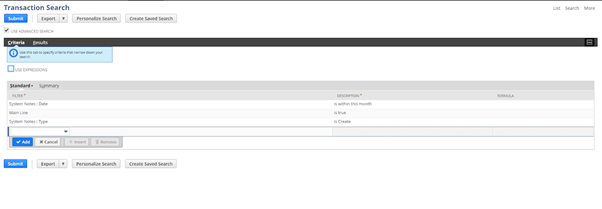
\includegraphics[scale=0.7]{resource/data.png}
    \caption{extracting data interface}
    \label{figure:saveSearch}
\end{figure}



\begin{lstlisting}[language=SQL, caption={equal to SQL}, label={lst:sqlNetSuite} ]
SELECT "Order Type", "Date","Period","Type","Document Number",
    "Name", "System Notes: Set by", "Created From", 
    "Applied to Transaction","Applying Transaction", 
    "System Notes: Role","System Notes: Set by"  
FROM "transaction"
WHERE "SYSTEM NOTE:DATE" 
    WITHIN "01.01.2021" AND 
           "09.02.2022" AND 
    "SYSTEM NOTES: TYPE" == "CREATE"
\end{lstlisting}

In Fig~\ref{table:dataformat} shows the data in CSV format. There are 10000 traces in the dataset where it shows only the trace 5. There are many activities in trace 5 i.e., Document ID and Period and Created from, timestamp . The trace 1 contains many sequences of activities. Likewise there are 10000 traces are populated using the transaction activities.

\begin{table}[htb]
\scriptsize %changing the font size
\begin{tabularx}{\textwidth}{|X|X|X|X|X|X|X|X|X|}
\hline
Internal ID & Date & Type & Document Number & Created From & Applied to Transaction & Applying Transaction & Role & Set by\\
\hline
1822448 & 01/02/2021 & Item Receipt &	37308 &	Purchase Order \#54527 &  &   & I.T.T. Stock Room & Employee \#1\\
\hline
1822449 & 01/02/2021 & Item Fulfillment &	52882 &	Sales Order \#60219 & Sales Order \#60219  &   & I.T.T. Stock Room & Employee \#1\\
\hline
1822454 &	31/01/2021 &	Journal &	4672 &	Invoice \#64932 &	Invoice \#64932 &	& Highlander Accountant &	Employee \#2 \\
\hline

\end{tabularx}
\caption{Data Format From NetSuite}
\label{table:dataformat}
\end{table}


Even log contains columns in table~\ref{table:dataformat} from left to right:
\begin{enumerate}
    \item  Internal ID: This is the unique ID for each activity from NetSuite databased ID
    \item Date: It is itemtamp for activity
    \item Type: The columns show different type of activity
    \item Document Number: The unique activity ID
    \item Created From: The columns shows that the activity created from another activity's ID and Type
    \item Appplied to Transactions (Applying Transaction): The next associated activity.
    \item Role: The role created or triggered the activity.
    \item Set by: The specific employed triggered the activity
\end{enumerate}

\subsection{Data Processing}
Data preprocessing is the efficient process to discover suitable attributes from the event log. Collection of sequence process in the event are extracted from the source list of activities and mentioned the related events and attributes of log. We have to concentrate important processes to maintain the efficiency in the source data set, i.e.
\begin{enumerate}
    \item Noise
    \item Incompleteness
\end{enumerate}

Noise: The incorrect event logs are removed from the dataset.
While extracting information from event log the various
sources can interleaf the information. The algorithm will
mislead the accuracy of the result. So the non-behavioral
information must be distinguished from the other data set and
retrieve the proper information.
Incompleteness: The unwanted and NAN attributes are produce noise in
the data process and mislead the control flow of the process
mining

\subsection{ProM Tool}
The information is collected and stored in database, it is
important to convert the data into XSLX format. ProM will accept the CSV file, so the dataset
of other format need to be changed to CSV file format using Python\ref{pythonCode}. The
CSV extension file is an input to the ProM that has to be
imported using the import option. The required attributes are
selected for process mining like activities and time of the
activities. We can filter the attributes which are used
particularly in the process.

\subsection{Event Log Preparation}

In our dataset, we have identified 10000 cases and have taken as the event log. Those one thousand tractions are directed to different events and 12000 events are traced in event history over there. The activities are segregated into 20 event classes. The mean values of these events are calculated based on cases. Fig~\ref{figure:promXESEvent} shows the number of cases, events and mean value of the given dataset. In 10000 traces the minimum and maximum values are traces in the Fig~\ref{figure:promXESEvent}. The total traces and by event trace are also mentioned in the diagram. This is the event log visualizer in the process mining. This visualizer helps to see the summary of the activity trace in the process. Log visualizer traces the event which is occurring starting and ending of the process. As well the activity sequence in each trace also identified in this

\begin{figure}[!htb]
    \centering 
    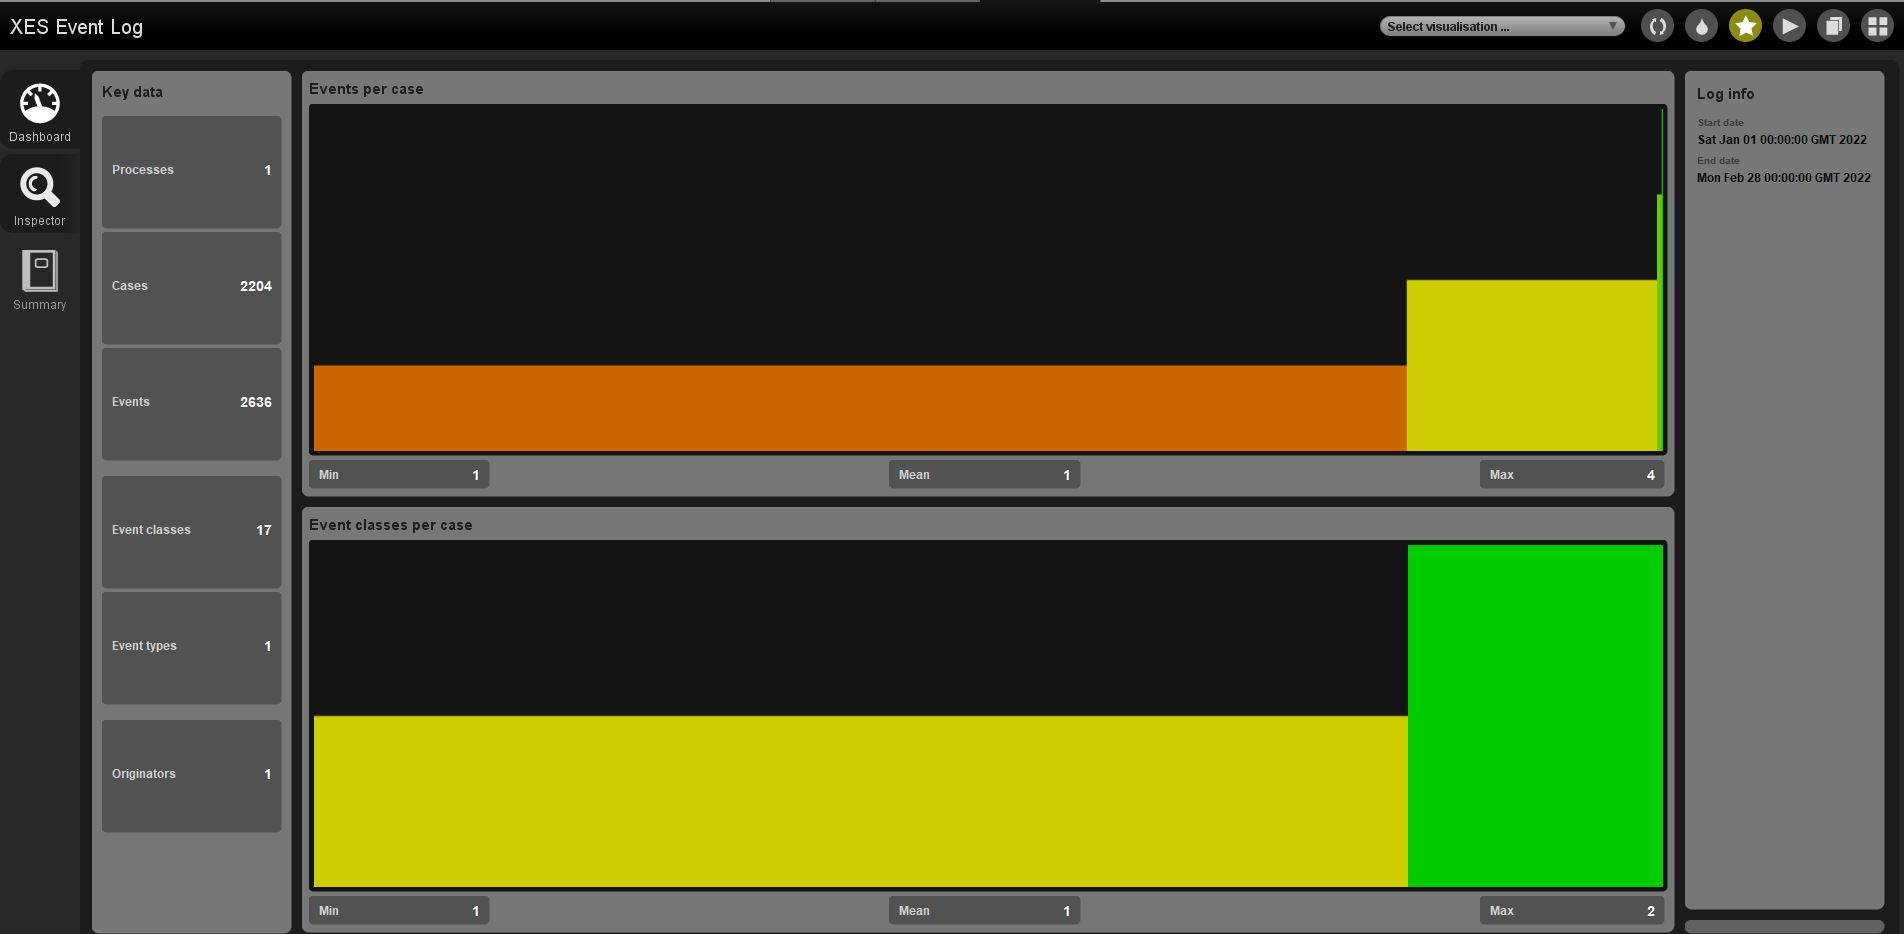
\includegraphics[scale=0.3]{resource/XESEventLog.JPG}
    \caption{ProM lite 1.3 XES Event Log Problems}
    \label{figure:promXESEvent}
\end{figure}

\subsection{Event Log Traces}
\begin{figure}[!htb]
        \centering 
    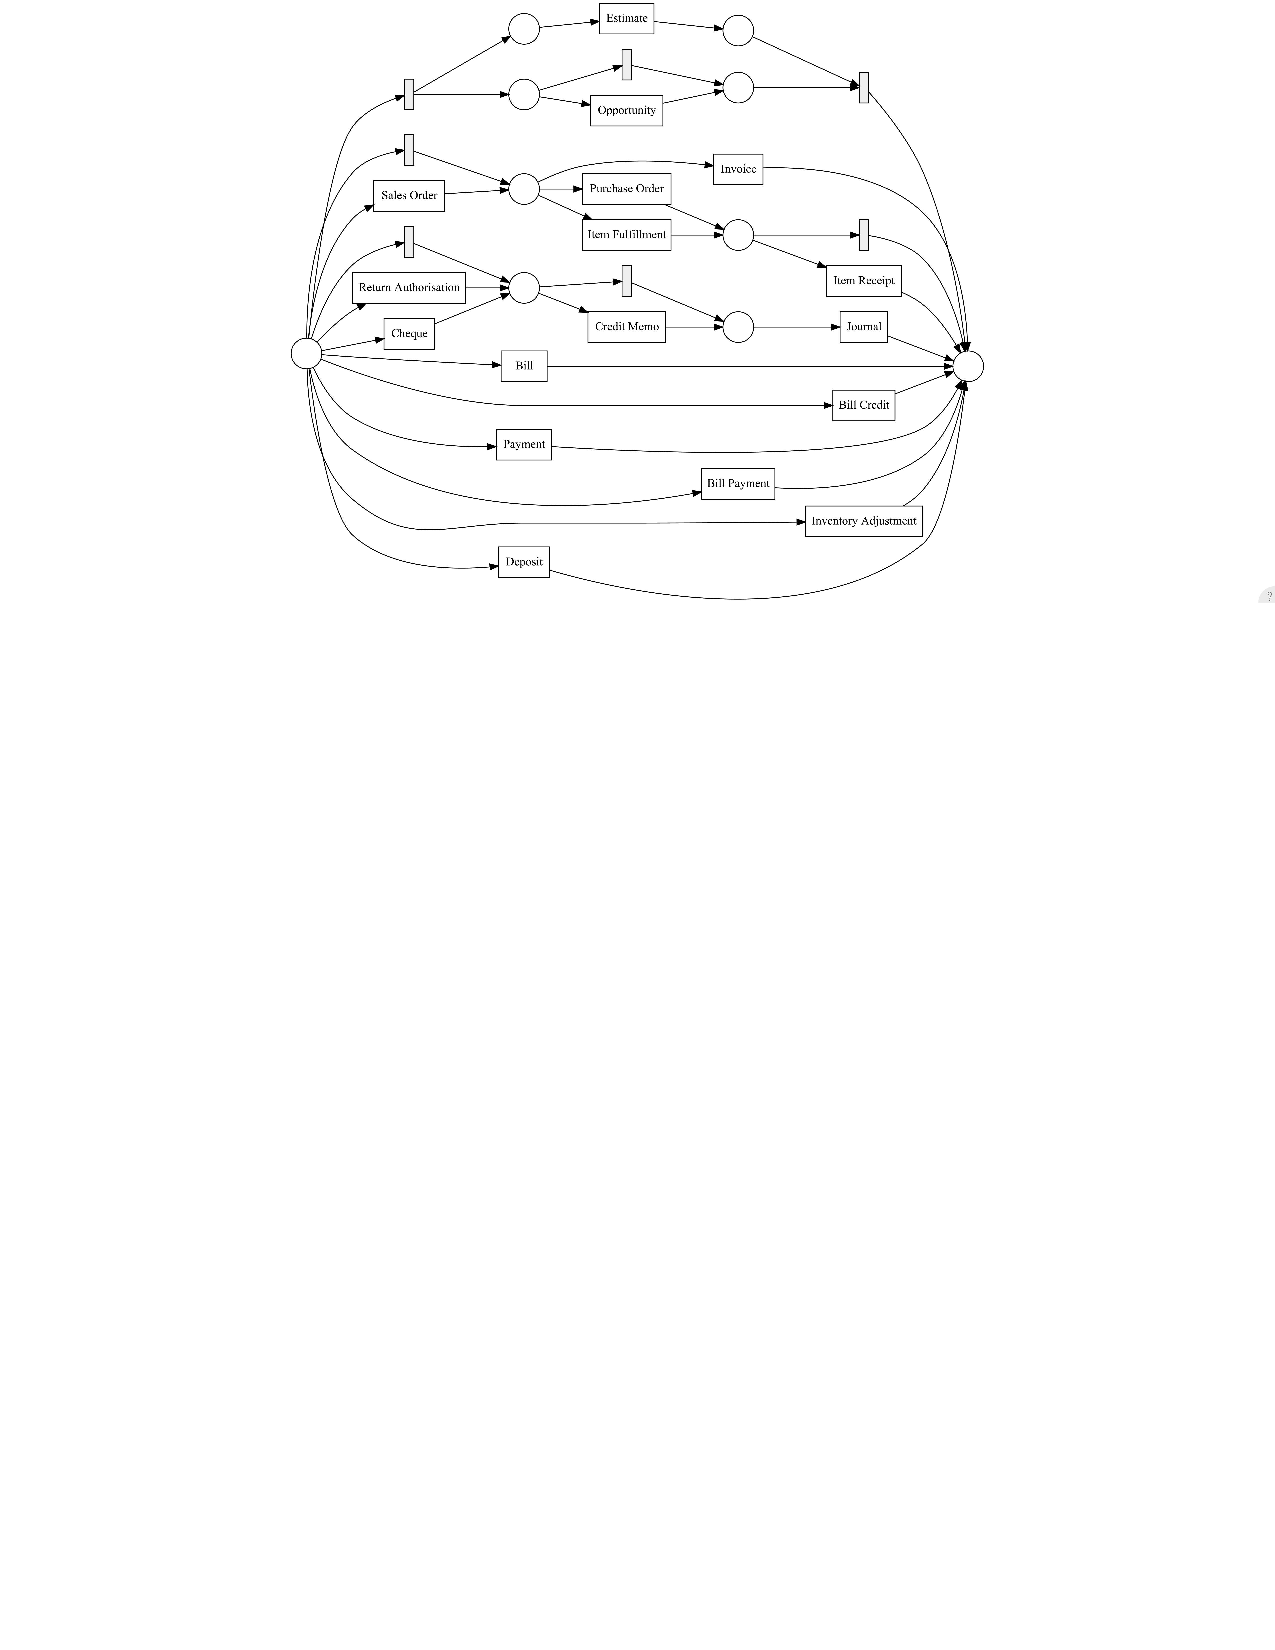
\includegraphics[width =\textwidth, trim =1cm 17cm 0cm 0cm, clip]{resource/problem2.pdf}
    \caption{ProM lite 1.3 Inductive visual Miner}
    \label{figure:eventLogTraces2}

\end{figure}

\subsection{Process Quality}

\subsection{Miner Algorithm}

\paragraph{Alpha miner}

The alpha-algorithm analyzes the event log to design graphs called patterns. The event log contains the concurrent activities in particular process that means the sequence of activities. The design follows the order of relation in between the activities. Finally alpha algorithm produces the petri net design as result. Our experiment, if activity d is followed by e but vice versa is not possible, then the algorithm confirms dependency relation between d and e. To reflect this dependency, the corresponding Petri net should have a place connecting d to e. We use ordering in between the relations to design the pattern in the event log.

Whenever the complex and frequent activity paths, produces spaghetti[27], that shows the complex structure. The graph determines the activity process flow of patients from start to end. The patient’s details are maintained in admin and the treatment activity and time stamp are mentioned in the process. There are many parallel processes going on and all are noted with time stamp. In alpha algorithm, the entire process will be shown as a graph[28]. Hence, this method which is used for real time applications, such as healthcare process are very helpful to the doctors, hospitals and patients for quick treatment with respect to processing time, waiting time, etc.

\paragraph{The Heuristics miner}
\paragraph{Inductive miner}
\paragraph{Fuzzy miner}






\section{Process mining tools}
\subsection{ProM}
ProM is an extensible framework that supports a wide variety of process mining techniques in the form of plugins. 
It is platform independent as it is implemented in Java, and can be downloaded free of charge. It provides different import data formats, like XES, XML, JSON.
\subsection{Apromore}
Apromore is an open-source process model repository. Its source code is available under the GNU Lesser General Public License.Apromore’s basic features include model import and export, version control and modeling support for a variety of languages, e.g., BPMN,
eEPC, YAWL, and Petri nets. It also supports CSV import. However, they required a format for CSV files 

\section{Source Code}

\lstinputlisting[language=Python,label={pythonCode},caption=Clean Data Source Code]{resource/Code/cleanData.py}